\documentclass[titlepage]{article}

\usepackage[letterpaper,margin=1in,footskip=0.25in]{geometry}
\usepackage[hidelinks]{hyperref}
\usepackage{fancyhdr}
\usepackage{csquotes}
\usepackage{tikz}
\usepackage[list=true]{subcaption}
\usepackage{graphicx}

\MakeOuterQuote{"}

\usetikzlibrary{knots}

\newcommand{\dq}[2]{``#1" (#2).}

\title{{\Huge\emph{The Knot Book}}\\[5pt]\textcolor{gray!60!black}{Notes}\vspace{-0.5em}}
\author{Steven Labalme}
\date{\today}

\begin{document}




\pagenumbering{gobble}
\maketitle



\pagenumbering{roman}
\tableofcontents
\listoffigures
\listoftables
\newpage



\pagenumbering{arabic}
\pagestyle{fancy}
\fancyhf{}
\rfoot{Labalme \thepage}
\renewcommand{\headrulewidth}{0pt}
\section{Introduction}\label{sse:intro}
\subsection{Introduction}
\begin{itemize}
    \item \textbf{Knot}: \dq{A knotted loop of string, except that we think of the string as having no thickness, its cross-section being a single point}{2}
    \item Do not distinguish between a `nice, even' knot and one that has been deformed through space.
    \item \textbf{Unknot}: \dq{The simplest knot of all\dots the unknoted circle}{2} \emph{Also known as} \textbf{trivial knot}. See Figure \ref{fig:circletrefoila}.
    \item \textbf{Trefoil knot}: \dq{The next simplest knot}{2} See Figure \ref{fig:circletrefoilb}.
    \begin{figure}[h!]
        \centering
        \begin{subfigure}{0.2\linewidth}
            \centering
            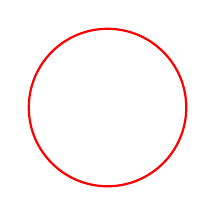
\begin{tikzpicture}
                \draw[red,thick] (0,0) circle (1cm);
            \end{tikzpicture}
            \caption{Trivial knot.}
            \label{fig:circletrefoila}
        \end{subfigure}
        \begin{subfigure}{0.2\linewidth}
            \centering
            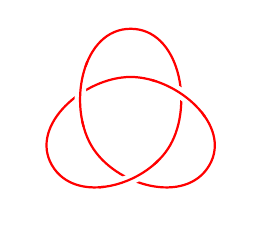
\begin{tikzpicture}
                \begin{knot}[
                    consider self intersections,
                    clip width=5
                ]
                    % could be defined with a combination of polar coordinates and foreach...
                    \strand[red,thick] (1,{3^0.5})
                        to [out=0,in=60] (1.5,0.25)
                        to [out=240,in=-60] (0,0)
                        to [out=120,in=180] (1,1.12)
                        to [out=0,in=60] (2,0)
                        to [out=240,in=-60] (0.5,0.25)
                        to [out=120,in=180] cycle
                    ;
                    \flipcrossings{1,3}
                \end{knot}
            \end{tikzpicture}
            \caption{Trefoil knot.}
            \label{fig:circletrefoilb}
        \end{subfigure}
        \caption{Projections of the two simplest knots.}
        \label{fig:circletrefoil}
    \end{figure}
    \item \textbf{Projection}: A picture of a knot, such as those in Figure \ref{fig:circletrefoil}.
    \begin{itemize}
        \item The same knots can have multiple projections (as they are deformed in space).
    \end{itemize}
    \item \textbf{Crossings}: The places in a projection where a knot crosses itself.
    \begin{itemize}
        \item The trefoil knot in Figure \ref{fig:circletrefoilb} is a \underline{three-crossing knot} because it crosses itself 3 times.
        \item Any one-crossing knot is trivial.
        \item \emph{Exercise 1.2}: Any two-crossing knot must be trivial because the simplest nontrivial knot is the trefoil knot, which has three crossings.
    \end{itemize}
    \item Atoms were originally thought to be tangles (knots) in the ether of the universe, but when chemists moved on, mathematicians took up knot theory. In the 1980s, biochemists began to see applications of knot theory in their research (see Section \ref{sse:biochemphys}).
    \item \textbf{Topology}: \dq{The study of the properties of geometric objects that are preserved under deformations}{6}
    \begin{itemize}
        \item Knot theory is a subfield of topology (see Section \ref{sse:topology}).
    \end{itemize}
    \begin{figure}[h!]
        \centering
        \includegraphics[width=0.7\linewidth]{Blender/CubeSphere.png}
        \caption{Deformation of a cube into a sphere.}
        \label{fig:cubesphere}
    \end{figure}
    \item Any knot can have a projection with as many crossings as desired.
    \item \textbf{Alternating knot}: \dq{A knot with a projection that has crossings that alternate between over and under as one travels around the knot in a fixed direction}{7}
    \begin{itemize}
        \item The trefoil is such a knot.
    \end{itemize}
    \item \emph{Exercise 1.7*}: By changing some of the crossings from over to under or vice versa, any projection of a knot can be made into a projection of the unknot$^[$\footnote{How can I \emph{show} something? How can I do these proofs? What kind of logic solves one of these?}$^]$. See Figure \ref{fig:knottotrivial}.
    \begin{figure}[h!]
        \centering
        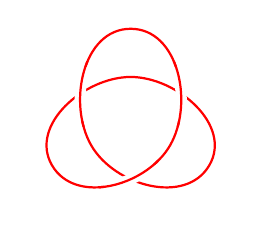
\begin{tikzpicture}
            \begin{knot}[
                consider self intersections,
                clip width=5
            ]
                \strand[red,thick] (1,{3^0.5})
                    to [out=0,in=60] (1.5,0.25)
                    to [out=240,in=-60] (0,0)
                    to [out=120,in=180] (1,1.12)
                    to [out=0,in=60] (2,0)
                    to [out=240,in=-60] (0.5,0.25)
                    to [out=120,in=180] cycle
                ;
                \flipcrossings{3}
            \end{knot}
        \end{tikzpicture}
        \caption{A projection of the unknot evoking the trefoil knot.}
        \label{fig:knottotrivial}
    \end{figure}
\end{itemize}


\subsection{Composition of Knots}
\begin{itemize}
    \item \textbf{Composition} (of two knots): \dq{A new knot obtained by removing a small arc from two knot projections and then connecting the four endpoints by two new arcs}{7}
    \begin{itemize}
        \item If two knots are designated $J$ and $K$, then their composition is denoted $J\#K$.
        \item Do not overlap the projections and choose two arcs that are on the outside to avoid new crossings.
        \item Make sure that the new arcs do not cross any of the the original knot projections or each other.
    \end{itemize}
    \item \textbf{Composite knot}: A knot that \dq{can be expressed as the composition of two knots, neither of which is the trivial knot}{8}
    \begin{itemize}
        \item This definition is analogous to composite integers, where an integer is \underline{composite} if it is the product of positive integers, neither of which is $1$.
        \item Similarly, if we compose any knot with the unknot, we get the same knot back.
    \end{itemize}
    \item \textbf{Factor knots}: \dq{The knots that make up the composite knot}{8}
    \item \textbf{Prime knot}: \dq{A knot [that] is not the composition of any two nontrivial knots}{9}
    \item The unknot, trefoil knot, and figure-eight knots are all prime (see Section \ref{sss:GenusSeifert}).
    \begin{itemize}
        \item The unknot is not composite for the same reason that 1 is not the product of two integers greater than 1.
    \end{itemize}
    \begin{figure}[h!]
        \centering
        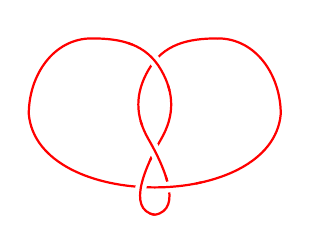
\begin{tikzpicture}[scale=0.8]
            \begin{knot}[
                clip width=5
            ]
                % Use looseness=# key to stretch out lengths!
                \strand[red,thick]       (0,0)
                    to [out=-85,in=-95]  (4,0)
                    to [out=90,in=0]     (3,1.2)
                ;
                \strand[red,thick]       (3,1.2)
                    to [out=180,in=60]   (1.9,0.7)
                    to [out=-120,in=120] (1.9,-0.4)
                    to [out=-60,in=10]   (2,-1.6)
                ;
                \strand[red,thick]       (2,-1.6)
                    to [out=170,in=-120] (2.1,-0.4)
                    to [out=60,in=-60]   (2.1,0.7)
                    to [out=120,in=0]    (1,1.2)
                    to [out=180,in=90]   (0,0)
                ;
                \flipcrossings{2,3}
            \end{knot}
        \end{tikzpicture}
        \caption{The figure-eight knot.}
        \label{fig:figure8knot}
    \end{figure}
    \item Similar to integers, \dq{a composite knot factors into a unique set of prime knots}{10}
    \newpage
    \item \emph{Exercise 1.8}: Using the appendix table, identify the factor knots that make up the composite knot in Figure \ref{fig:compos1}.
    \begin{figure}[h!]
        \centering
        \includegraphics[width=0.15\linewidth]{Blender/compos1.png}
        \caption{The composite knot.}
        \label{fig:compos1}
    \end{figure}
    \begin{itemize}
        \item \textsc{Figure out when knot cord arrives.}
    \end{itemize}
    \item \emph{Exercise 1.9}: Show that the knot in Figure \ref{fig:compos2} is composite.
    \begin{figure}[h!]
        \centering
        \begin{subfigure}[b]{0.3\textwidth}
            \centering
            \includegraphics[width=0.5\textwidth]{Blender/compos2.png}
            \caption{The composite knot.}
            \label{fig:compos2a}
        \end{subfigure}
        \begin{subfigure}[b]{0.3\textwidth}
            \centering
            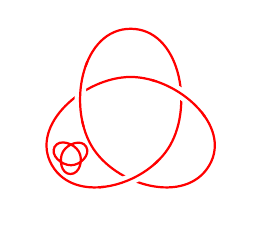
\begin{tikzpicture}
                \begin{knot}[
                    clip width=5,
                    consider self intersections
                ]
                    % Why don't polar coordinates mesh with figures?
                    \strand[red,thick] (1,{3^0.5})
                        to [out=0,in=60] (1.5,0.25)
                        to [out=240,in=-60] (0,0)
                        to [out=120,in=180] (1,1.12)
                        to [out=0,in=60] (2,0)
                        to [out=240,in=-60] (0.5,0.25)
                        to [out=120,in=180] cycle
                    ;
                    \flipcrossings{1,3}
                \end{knot}
                \begin{knot}[
                    clip width=5,
                    consider self intersections,
                    rotate=60,
                    scale=0.2,
                    xshift=0.1cm,yshift=-1.3cm
                ]
                    % Why don't polar coordinates mesh with figures?
                    \strand[red,thick] (1,{3^0.5})
                        to [out=0,in=60] (1.5,0.25)
                        to [out=240,in=-60] (0,0)
                        to [out=120,in=180] (1,1.12)
                        to [out=0,in=60] (2,0)
                        to [out=240,in=-60] (0.5,0.25)
                        to [out=120,in=180] cycle
                    ;
                    \flipcrossings{1,3}
                \end{knot}
            \end{tikzpicture}
            \caption{Factors.}
            \label{fig:compos2b}
        \end{subfigure}
        \caption{Factorization of a `double trefoil.'}
        \label{fig:compos2}
    \end{figure}
\end{itemize}




\end{document}



% \subsection{Reidemeister Moves}
% \begin{itemize}
%     \item \dq{hi}{\#\#}
% \end{itemize}


% \subsection{Links}
% \begin{itemize}
%     \item \dq{hi}{\#\#}
% \end{itemize}


% \subsection{Tricolorability}
% \begin{itemize}
%     \item \dq{hi}{\#\#}
% \end{itemize}


% \subsection{Knots and Sticks}
% \begin{itemize}
%     \item \dq{hi}{\#\#}
% \end{itemize}